\documentclass[a4paper,11pt]{article}
\usepackage{sbpo-template}
\usepackage[english]{babel}
\usepackage[utf8]{inputenc}
\usepackage{amsmath,amssymb}
\usepackage{url}
\usepackage[square]{natbib}
\usepackage{indentfirst}
\usepackage{fancyhdr}
\usepackage{colortbl}
\usepackage{amsmath,amsthm}
\usepackage{amssymb}
\usepackage{mathtools}
\newcommand\crule[3][black]{\textcolor{#1}{\rule{#2}{#3}}}
\usepackage{graphicx}
\usepackage{hyperref}
\hypersetup{
  colorlinks=true,
  linkcolor=blue,
}
\newcommand{\midtilde}{\raisebox{-0.25\baselineskip}{\textasciitilde}}
\usepackage[table,xcdraw]{xcolor}
\usepackage[acronym]{glossaries}
\pagestyle{fancy}
\usepackage{tikz}
\fancyhf{}
\fancyhead[C]{
\includegraphics[width=\textwidth]{cabecalho_sbpo.png}}
\renewcommand{\headrulewidth}{0pt}
\setlength\headheight{101.0pt}
\addtolength{\textheight}{-101.0pt}
\setlength{\headsep}{-5mm}

\newacronym{ew}{EW}{Epidemiological Week}
\newacronym{parp}{PARP}{Prize-collecting Arc Routing Problem}
\newacronym{dparp}{Dengue-PARP}{Dengue Prize-collecting Arc Routing Problem}
\newacronym{ilp}{IP}{Integer Programming}
\newacronym{ml}{ML}{Machine Learning}

\definecolor{lgr}{HTML}{C0C0C0}
\definecolor{gr}{HTML}{9B9B9B}

\begin{document}

\title{A Prize Collecting approach for the Dengue Arc Routing Problem} 

\maketitle
\thispagestyle{fancy}

\author{
\name{Carlos V. D. Araujo}
\institute{Filia\c c\~ao}
\iaddress{Endere\c co da Institui\c c\~ao}
\email{e-mail}
}

\author{ 
\name{Segundo Autor}
\institute{Filia\c c\~ao} 
\iaddress{Endere\c co da Institui\c c\~ao}
\email {e-mail}
}

\vspace{8mm}
\begin{resumo}
Este modelo resume as normas de formata\c c\~ao para os trabalhos completos a serem publicados
nos Anais do LII SBPO. T\'\i tulo, filia\c c\~ao, resumo e palavras-chave devem repetir fielmente
o que foi informado quando o autor cadastrou o artigo atrav\' es do sistema de submiss\~ao.
O Resumo deve ter no m\' aximo 150 palavras.
 \end{resumo}

\bigskip
\begin{palchaves}
Primeira, Segunda, Terceira.

\bigskip
\noindent{T\'opicos (indique, em ordem de PRIORIDADE, o(s) t\'opicos(s) de seu artigo) }
\end{palchaves}


\vspace{8mm}

\begin{abstract}
This document presents the format for full papers to be published in the Annals of the LII SBPO.
Title, affiliation, abstract and keywords must be exactly the same as the author informed when registered the paper through the submission system. 
The Abstract must not exceed 150 words.
\end{abstract}

\bigskip
\begin{keywords}
First keyword. Second keyword. Last keyword.

\bigskip
\noindent{Paper topics (indicate in order of PRIORITY the paper topic(s))}
\end{keywords}

 
\newpage
\section{Introduction}


According to the Pan American Health Organization  (PAHO), in the year of 2021 a
total  of  1.324.108  cases  of  arbivoral diseases  were  reported.  Of  those,
1.173.674 ($89\%$) were dengue cases, 131.630 were chikungunya cases, and 18.844
were  Zika. Between  the \gls{ew}  1 and  the \gls{ew}  19 of  2022, a  total of
1.279.724 arbivoral  disease already been  reported, in which Brazil  appears in
first position as the country with  the largest number of dengue reported cases,
achieving a total of 1.114.758 ($90.9\%$) \citep{paho-1}.

The  prevention,  control,  and  combat   of  diseases  caused  by  arboviruses,
especially  dengue, has  been subject  of great  concern worldwide,  as it  is a
reemerging disease caused by the transmission of Den  1, Den 2, Den 3, and Den 4
viruses  through  the {\em  Aedes  aegypt}  and  {\em Aedes  albopictus},  which
proliferates in  the tropical  regions of  the world,  comprising more  than 1.8
billions of people susceptible to being infected \citep{negreiros-2020}.

The dengue virus needs a biological vector to be transmitted. The control of the
mosquito can be done in two  ways: eliminating adult mosquitoes, and eliminating
the larval  breeding grounds. In addition  to precaution, where the  focus is to
make the population aware and eliminate  possible recipients that could serve as
breeding grounds for mosquitoes, chemical control is the most used approach. The
chemical  control  consists in  the  use  of  chemical substances  (for  example
insecticide) for vector control in the larval and adult stages.

The use of  insecticides in public health is based  on technical and operational
standards,  that derived  from a  group of  experts in  pesticides of  the World
Health  Organization  (WHO), which  recommends  the  active ingredients  of  the
products and recommends the doses for the various types of available treatments.
The rational and safe use in  vector control activities is essential, given that
their indiscriminate  use determines environmental  impacts, in addition  of the
vector developing  resistance to the  products. An emergency approach  to reduce
the adult mosquito  population, used in case of epidemics  or endemics mainly in
urban areas,  is to apply  insecticide using  a nebulizer equipment  attached to
vehicles, which  we call throughout  this work  as spraying vehicle,  see Figure
\ref{fig:nebulizer}.

\begin{figure}[!ht]
  \centering
    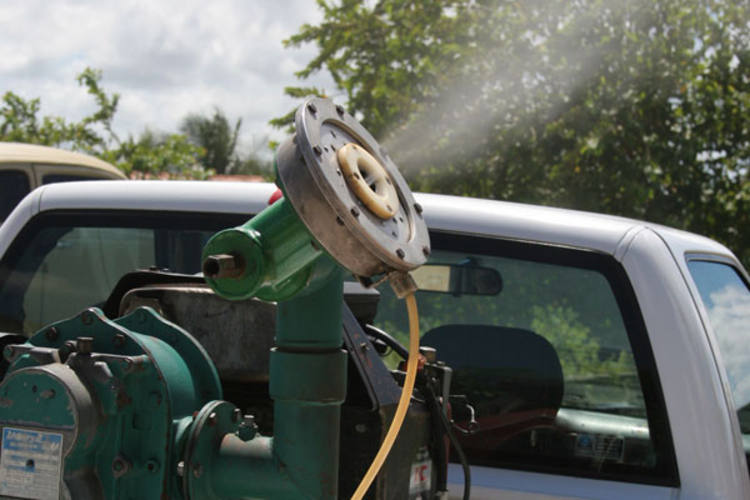
\includegraphics[scale=0.4]{fumace.jpg}
    \caption{Nebulizer equipment attached to vehicle. }
    \label{fig:nebulizer}
\end{figure}

Spraying vehicles  are very useful for  the control of outbreaks  and epidemics,
due to its high performance, 80 to 160 blocks per day depending of the equipment
model, however it  is not recommended in situations where  the transmission need
to be blocked. These applications must be constantly supervised to guarantee the
indicated insecticide dosage in each visited  street, since there is a series of
operational   factors,  such   as   the  equipment   flow   and  vehicle   speed
\citep{brasil-dept-helth:2009}. In  order for the spraying  vehicle applications
to have the desired effectiveness, it must  be realized in a period with correct
conditions to  maintain the insecticide  cloud moving  close to the  ground. The
thermal inversion is  generally produced in the morning, after  the sunrise, and
in the  afternoon, just before  sunset, these moments  are optimal to  apply the
insecticide with the spraying vehicle.

The sprayed insecticide has no residual  effect and it is strongly influenced by
wind and  obstacles along the  streets. The best  results are achieved  when the
most dense  insecticide cloud  is at  a distance of  up to  100 meters  from the
equipment.  As this  distance  is  crossed, the  effectiveness  decreases, as  a
consequence of droplet drift influenced by  factor of the environment. The cloud
dispersion is illustrated in Figure \ref{fig:dispersion}.

\begin{figure}[!ht]
  \centering
  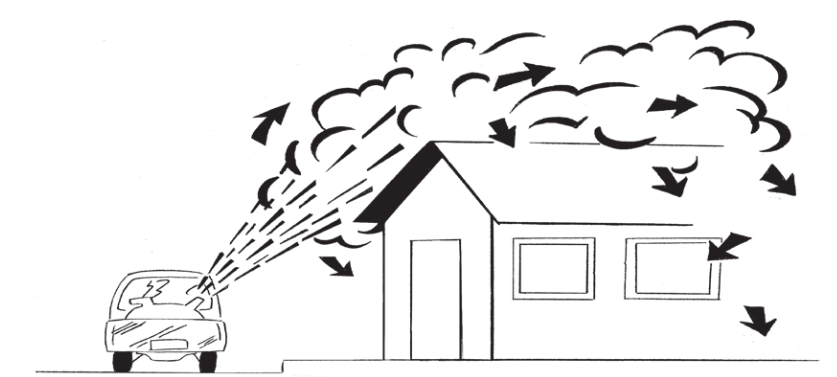
\includegraphics[scale=0.4]{cloud-dispersion.png}
  \caption{Cloud dispersion of the application.}
  \label{fig:dispersion}
\end{figure}

The instructions about the insecticide application method are generally based on
the  ideal conditions  of topology,  structure  of the  locality, and  favorable
winds. The operation  is often harmed by unpaved roads,  presence of high walls,
and  high vegetation,  in additions  to  headwinds. Such  this, the  application
methodology must  consider these limitations  in order  to obtain a  good impact
over the  vector population. The  vehicle must  travel around each  block before
starting the next one, as show in Figure \ref{fig:travel-pattern}.

\begin{figure}[!ht]
  \centering
  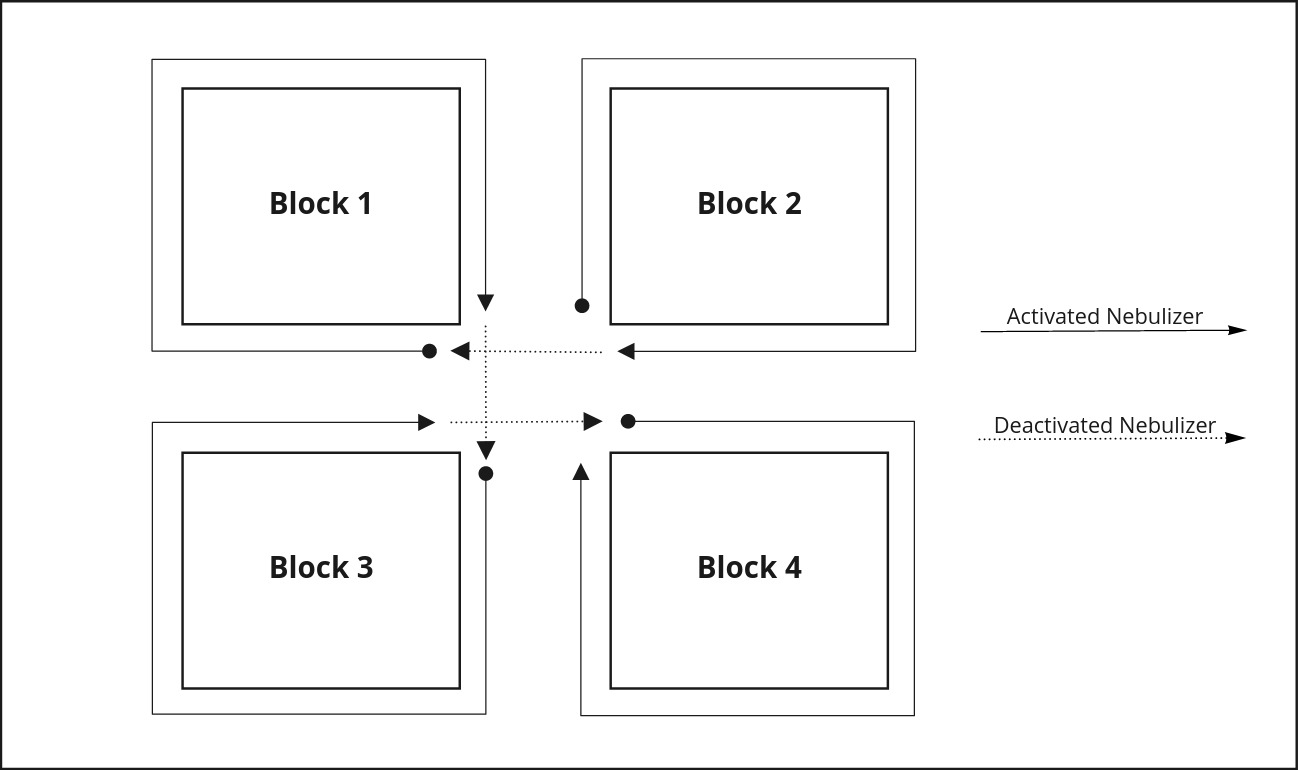
\includegraphics[scale=0.23]{visit-pattern.jpg}
  \caption{Vehicle pattern with nebulizer.}
  \label{fig:travel-pattern}
\end{figure}


The complexity of the process of prevention and control of the disease is large,
involving  only  in  Brazil,  annual   expenses  exceeding  R$\$$  1.6  billions
\citep{negreiros-2020}.  Such  resources could  be  better  used if  the  dengue
logistics was more  effective, and use the tools of  operations research. To the
best of our knowledge,  we are the first to introduce  the \gls{dparp}, which is
the problem of create routes to  spraying vehicles as a \gls{parp} with resource
constraints.  \gls{parp}s are  arc routing  problems where,  in addition  to the
cost, there is a profit function that must  be taken into account when an arc is
serviced \citep{araoz:2006}. In \gls{dparp}, each arc  of the block has a profit
value  that is  related to  the number  of dengue  cases, it  is considered  the
block-visit pattern described in  Figure \ref{fig:travel-pattern}, and limits of
time and insecticide. The  goal of the \gls{dparp} is to  maximize the profit in
order to  create a route that  cover a set  of streets/blocks. In this  work, we
formulated the  \gls{dparp} as a  \gls{ilp} and  test the model  using instances
based on real maps, containing real notified cases.

This work is  organized as follows. In  the next section we present  a review of
the  literature on  machine learning  and operations  research tools  applied in
dengue context.  Section \ref{sec:formulation}  introduces an \gls{ilp}  for the
\gls{dparp}. Section  \ref{sec:instance-generation} explains how  instances were
generated to validate the methodologies. Section \ref{sec:computational-results}
reports the computational  results. Finally, we make our  concluding remarks and
discuss some perspectives for future work in the last section.

\section{Related Work} \label{sec:related-work}

An extensive number  of works in the  literature use \gls{ml} in  the context of
dengue~\citep{shakurat:2015,shakil:2015,hair:2019,sarma:2020,appice:2020}. Some
of  the main  problems  addressed are  generate dengue  diagnoses  based on  the
patient's symptoms  and clinical patterns,  distinguish dengue and its  types in
the early stage of disease progression  and, dengue fever predictions in certain
regions  based on  a  set of  factors, such  as  precipitation, rain,  humidity,
temperature, and others.

\cite{lowe:2015} presented a  modeling procedure to quantify the  added value of
including  climate  information in  a  dengue  model  for  the 76  provinces  of
Thailand,  from  1982-2013  providing  decision  support  systems.  The  authors
considered a set  factors that have a statistically  significant contribution to
the relative  risk of  dengue in  the following months.  The system  provided an
advanced warning that enable the implementation of a more effective surveillance
system.  According  to  the  authors,  the model  framework  presented  here  is
extremely flexible and could be  applied in any geographical setting, generating
a  more global  approach  to assessing  the impact  of  climate variability  and
climate change on dengue risk.

\cite{bannwart-sbpo:2013,bannwart:2013}   proposed   numeric  techniques   using
genetic  algorithm  to solve  the  control  model  applied  to the  problems  of
combating dengue,  in which the  goal is to minimizes  the cost of  the chemical
control  (insecticide) and  genetic  (liberating sterile  males  in the  natural
environment). These works  assumes that the mortality rate of  the mosquitoes is
strongly  related  to the  investment  in  control approaches.  The  experiments
considered a time period  of 120 days and the results  indicated that the amount
of insecticide used was high considering the other approaches cited in the work,
however  the authors  presented an  analysis  considering each  control and  the
impact on the rate of reduction in the mosquito population.

\cite{cantane:2015} presented an experiment to  obtain the estimate rate used in
a  mathematical  model. The  mosquito  population  was conducted  under  optimal
conditions, simulating favorably  environment for its grow. Life  cycle data was
collected  daily, and  all  estimated  rates used  in  the  equation system  are
computed. It is  notorious that, without a control action,  the population could
highly  increase in  a short  amount  of time.  The results  of the  experiments
provide estimates of  the life cycle of the mosquitoes  are in perfect condition
in nature and the model allows to  measure a approximate number of mosquitoes in
the nature for this scenario.

The author of  \cite{dosreis:2018,florentino:2018,florentino-b:2018} presented a
set  of  methodologies for  dengue  control,  such  as mathematical  model  that
describes the population  dynamics of the Aedes aegypti, and  designed a generic
control law for the mosquito  population through exact linearization techniques.
Some heuristics  such as  Genetic Algorithm (GA)  in which the  main goal  is to
establishing  optimal strategies  using  an integration  of  different types  of
control  and  a Variable  Neighborhood  Search  (VNS) that  determine  optimized
control strategies  for the  aquatic phase,  producing a  lower cost  control to
reduce the mosquito  population. Some advantages presented are  that the control
in  aquatic phase  reduces  the environment  impact and  the  need for  chemical
control in large  scale. The results obtained by  computer simulations indicated
that  the presented  methodologies has  great potential  as a  tool for  support
decision maker against arboviroses.

The works of \cite{negreiros:2008,negreiros:2011,negreiros-2020}, to the best of
our knowledge, are the only papers that apply operations research techniques for
the context  of routing  problem along  with the  mosquito control.  These works
focuses on the computational tool called Web Dengue, aimed at helping the dengue
control managers providing  a better visualization of the  problem dimension and
better coordination of control procedures.  Among the methodologies presented in
\cite{negreiros:2008,negreiros:2011},   the   authors    developed   a   integer
programming  formulation  to compute  a  periodical  scheduling of  vehicles  in
determined areas. Also, in \cite{negreiros:2011} was developed a GRASP heuristic
to create routes for the vehicles with nebulizer, and the proposed algorithm was
applied  in a  instance  corresponding  to the  location  of  Praia de  Iracema,
Fortaleza.

\section{Mathematical Formulation for Dengue-PARP} \label{sec:formulation}

Consider a weighted, connected, and directed graph $G = (V, E)$, being $V = \{1,
\dots, n\}$ the  set of $n$ vertices, $E =  \{(i, j): i \text{ and }  j \in V, i
\neq j\}$ the set of $m$ edges. A block, in the \gls{dparp}, can be defined as a
cycle $C$ such that the edges $(i, j) \in C$ are in clockwise order. The set $B$
contains all blocks  of the instance, and each  vertex $i \in V$, that  is not a
deadend, belongs to at least one block, while  each edge $(i, j) \in E$ is in at
most one  block. In order to  allows the route starts  and end in any  vertex of
$G$, it is necessary to change $V$  to $V'$ by adding two artificial vertices, a
source $s$ and a  target $t$. It is also necessary add a  set of edges such that
$E' = E  \cup \{(s, u), (u, t)\},  \forall u \in V$. The notation  $B(i)$ is the
set of  blocks in which $i$  belongs, and $V(b)$ is  the set of vertices  in the
block $b$.

Each edge of $G$ contains two associated values: number of notified dengue cases
and distance in meters.  We set the \gls{dparp} entry as a  tuple ($G(V, E'), s,
t, B, \lambda,  \xi, f^T, f^I, i_{max}, T_{max}$), where  each edge contains the
values  of dengue  cases  ($\lambda$),  and distance  ($\xi$).  Consider a  time
function $f^T$ that  compute the time to  travel in a edge  ($f^T_{ij}$) and the
time to visit all  the edges of a block ($f^T_b$).  The function $f^I_b$ compute
the amount of insecticide used to spraying a block. Lastly, consider the maximum
amount of insecticide  available ($I_{max}$), and the maximum time  of the route
($T_{max}$).

A feasible route of \gls{dparp} can omit the cycles that make up a block, i. e.,
if the model consider  a block as sprayed, the route must  contains at least one
vertex from the block visited by the route. This approach takes advantage of the
nebulizer pulverization pattern presented for  this problem, that must cover all
the  edges  before  start  to  nebulize   another  block.  Next,  we  present  a
single-vehicle \gls{ilp} formulation for the \gls{dparp}.

\newpage
\subsection{Single-vehicle IP formulation}

Define the following variables:

\begin{itemize}
  \item $x_{ij}$: A binary variable that indicates whether the edge $(i, j) \in
    E'$ belongs to the route from $s$ to $t$;
  \item $y_{ib}$: A binary variable that is valued 1 if the vertex $i \in V$ is
    used as start point to spraying the block $b \in B(i)$; 
\end{itemize}
With these variables, the \gls{dparp} \gls{ilp} formulation reads:

\begin{align}
  \max & \sum_{i \in V} \sum_{b \in B} \lambda_b y_{ib} - \sum_{ij \in E} x_{ij} & \label{eq:of}\\
  \nonumber \text{subject to:} & & \\
       & \sum_{j \in V'\backslash \{t\}} x_{sj} = 1 & \label{eq:s-all} \\
       & \sum_{j \in V'\backslash \{s\}} x_{jt} = 1 & \label{eq:all-t} \\
       & \sum_{j: (i, j) \in E'} x_{ji} - \sum_{j: (i, j) \in E'} x_{ij} = 0 & \ \forall i \in V \label{eq:flow-conservation} \\
       & \sum_{(i, j) \in A'} f^T_{ij} x_{ij} + \sum_{i \in V} \sum_{b \in B} f^T_b y_{ib} \leq T_{\max} & \label{eq:max-time} \\
       & \sum_{i \in V'} \sum_{b \in B} f^I_b y_{ib} \leq I_{\max} & \label{eq:max-insecticide} \\
       & \sum_{i \in V(b)} y_{ib} \leq 1 & \ \forall b \in B \label{eq:max-attend} \\
       & \sum_{(i, j) \in A} x_{ij} \geq y_{ib} & \ \forall i \in V(b), b \in B \label{eq:in-path} \\
       & \sum_{(i, j) \in (S, \bar{S})} x_{ij} \geq y_{ib} & \ \forall S \subseteq V, i \in S, b \in B(i) \label{eq:subtour-elimination} \\
       & x_{ij} \in \{0, 1\} & \ \forall (i, j) \in E' \label{eq:dom-x} \\
       & y_{ib} \in \{0, 1\} & \ \forall i \in V, b \in B. \label{eq:dom-y} 
\end{align}

Each feasible solution for the \gls{ilp} model is a route starting at vertex $s$
and ending  in $t$  obeying the  limits of time  and insecticide.  The objective
function  \eqref{eq:of} maximizes  the profit  of each  edge in  a block,  while
minimizes       the      number       of      used       edges.      Constraints
\eqref{eq:s-all}-\eqref{eq:flow-conservation} enforces flow conservation at each
vertex. The constraints  \eqref{eq:max-time} limit the maximum time  used in the
route,  considering  a  different  velocity to  spraying  a  block.  Constraints
\eqref{eq:max-insecticide}   limits  the   amount  of   insecticide  used.   The
constraints \eqref{eq:max-attend} and \eqref{eq:in-path} ensure that at most one
vertex is used as start point to spraying  a block, and this vertices must be in
the   final  route.   Constraints  \eqref{eq:subtour-elimination}   are  subtour
elimination, ensuring the connectivity of the edges  in route when it is used to
spraying at  least one block. Constraints  \eqref{eq:dom-x}-\eqref{eq:dom-y} set
the domain of the variables.

\section{Instance Generation} \label{sec:instance-generation}

The first  step in generating instances  for the \gls{dparp} is  the creation of
roads and  highways. This work  adopted the maps  available in the  project open
Street Maps (OSM) \citep{haklay:2008}, which  is a collaborative mapping project
to create a free  and editable map of the world. Since  OSM allows returning GPS
coordinates of  each vertex, we  use this information  to create the  map blocks
cycles in clockwise orientation, since the  nebulizer in the vehicle always have
to  point to  right and  must cover  all  the streets  of a  block before  start
visiting the next.

The set  of instances  contains 39  instances based on  notified cases  from the
cities of  Alto Santo and  Limoeiro do  Norte, in the  state of Ceará  - Brazil.
These  notification were  obtained from  the Information  System for  Notifiable
Diseases (SINAN) \citep{laguardia:2004}, from  the years of 2015-2021, including
information about addresses  of the patients. The addresses were  applied in the
library  OSMnx \citep{boeing:2017}  in order  to obtain  geocodes (latitude  and
longitude),  and mapping  it to  blocks  as the  number  of cases  in the  edges
(streets). The OSMnx receives as input a  radius size to create the graph from a
map, the edges are the streets of  the map and the vertices are the intersection
of  two or  more streets,  as  shown in  Figure \ref{fig:graph-examples},  where
Figures (a)  and (b) are example  graphs obtained from Alto  Santo and Limoeiro,
respectively, with  radius value equal to  1000. Also, it is  necessary that the
address sought has been reported in  OSM to be possible retrieve the geolocation
data. After these steps, we can define each  block of the graph as a polygon and
execute an  algorithm that verifies  if the  point (geolocation) belongs  to any
polygon (block).

\begin{figure}[!ht]
  \begin{minipage}[c]{.6\textwidth}
    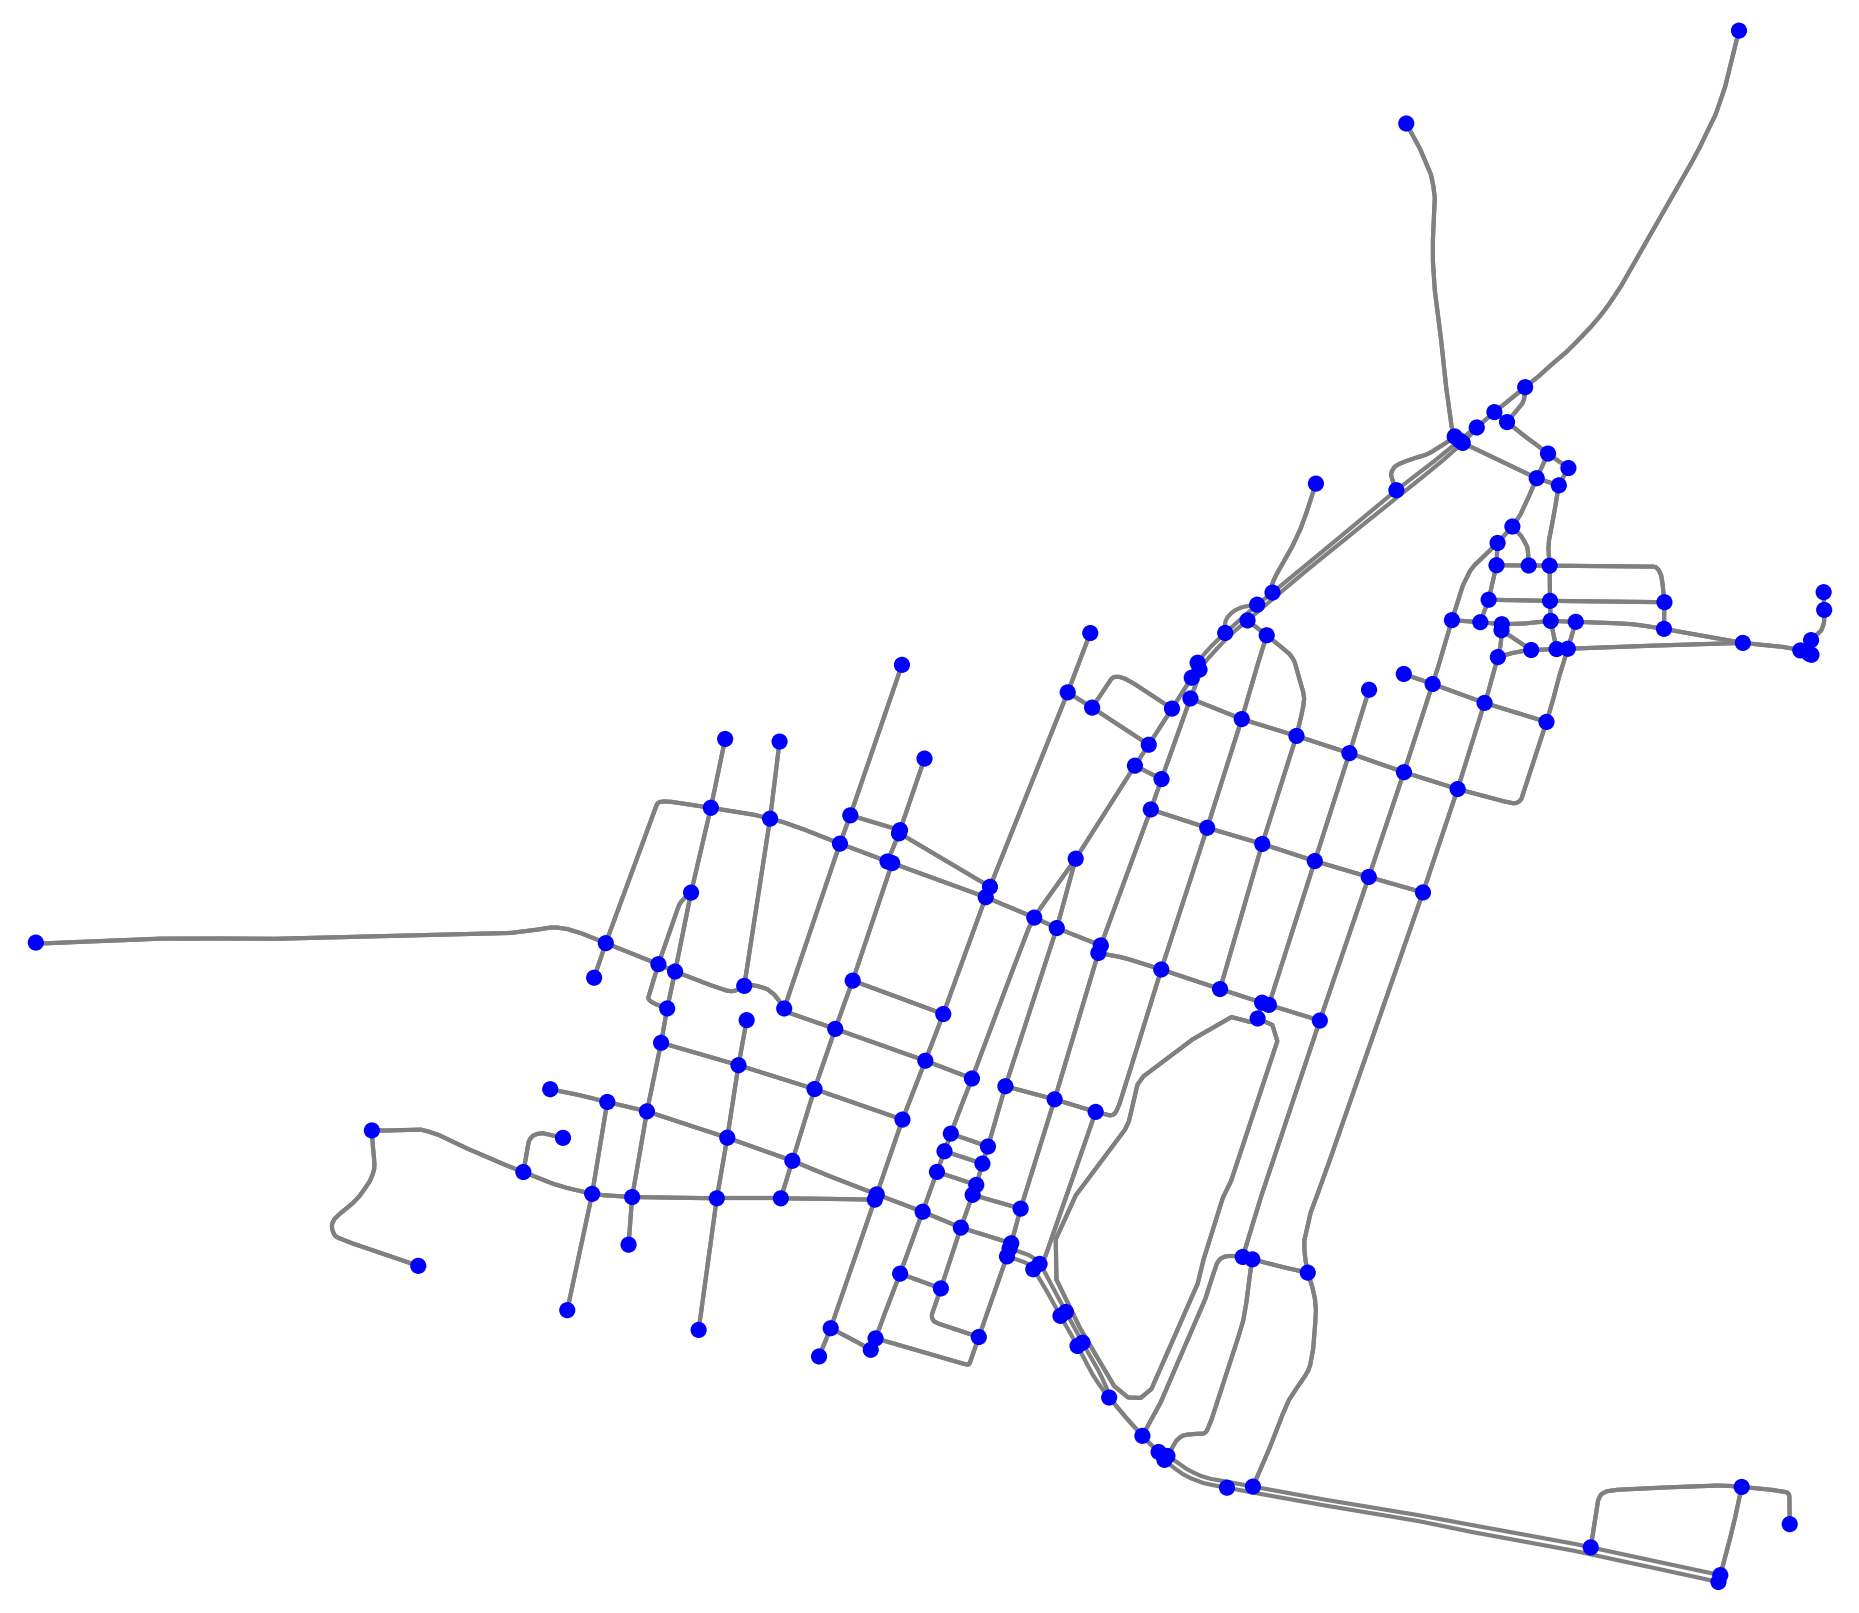
\includegraphics[width=6cm, height=6cm]{graph-alto-santo.png} \\
    (a) Example graph of Alto Santo.
  \end{minipage}
  % \quad
  \begin{minipage}[c]{.6\textwidth}
    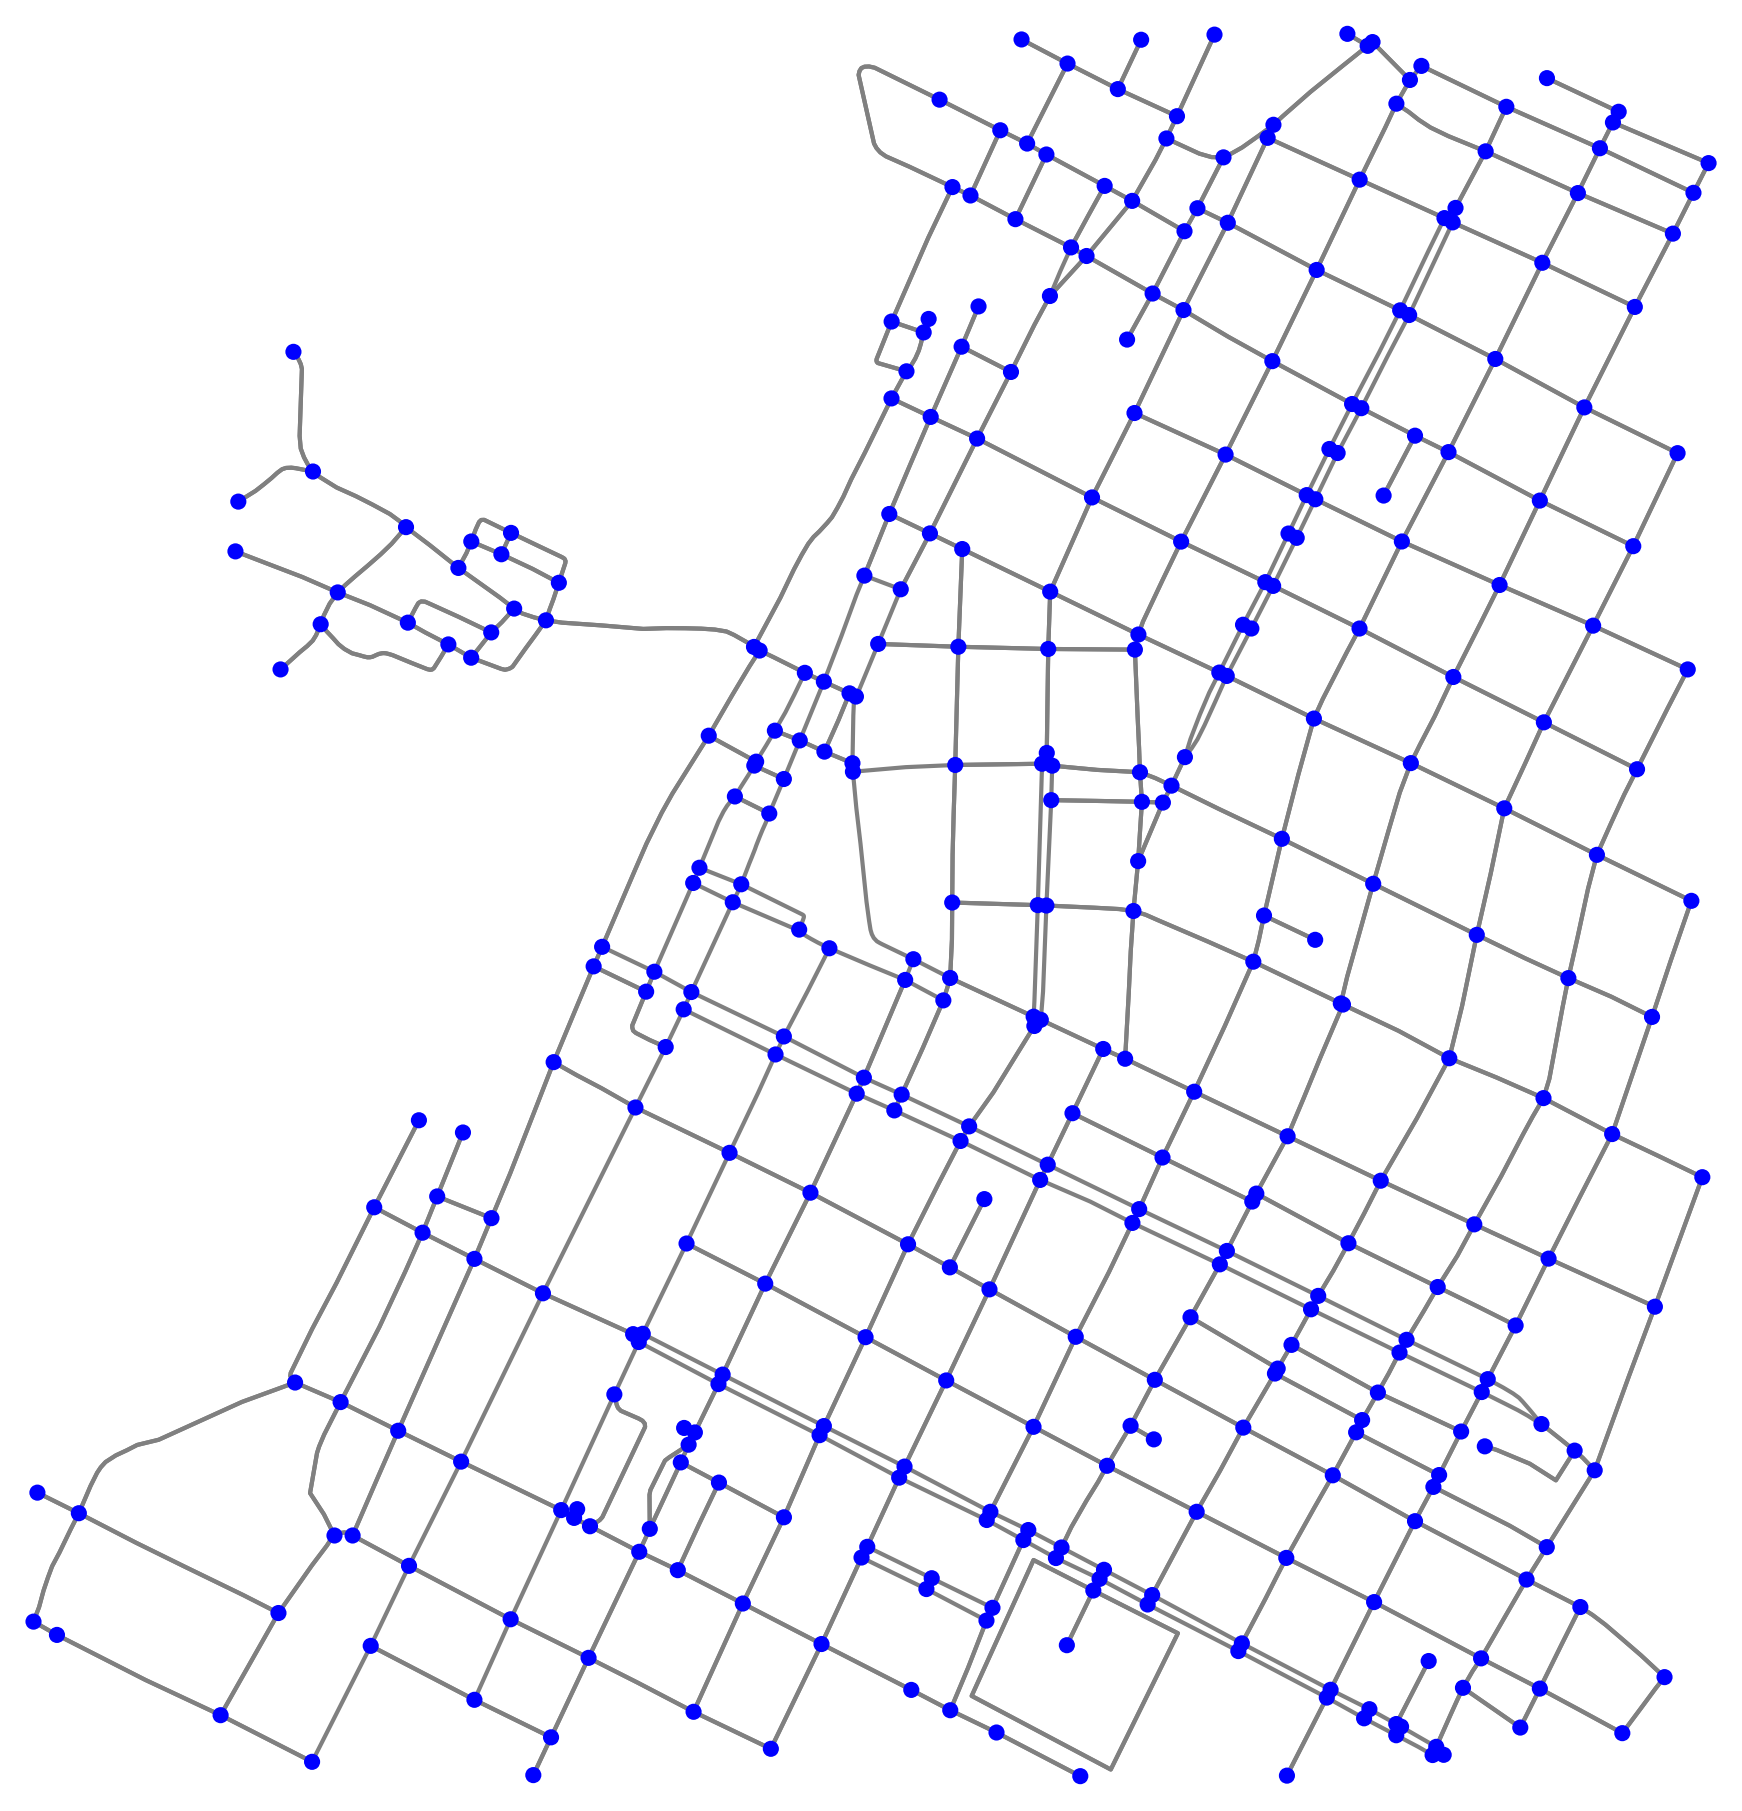
\includegraphics[width=6cm, height=6cm]{graph-limoeiro.png} \\
    (b) Example graph of Limoeiro.
  \end{minipage}
  \caption{\label{fig:graph-examples} Example of graphs with radius 1000.}
\end{figure}
% Please add the following required packages to your document preamble:
% \usepackage{graphicx}
% \begin{table}[!ht]
% \centering
% \small{%
% \begin{tabular}{lrrrrr}
% \hline
% \multicolumn{1}{c}{\textbf{instance}} &
%   \multicolumn{1}{c}{\textbf{$|V|$}} &
%   \multicolumn{1}{c}{\textbf{$|A|$}} &
%   \multicolumn{1}{c}{\textbf{$|B|$}} &
%   \multicolumn{1}{c}{\textbf{\begin{tabular}[c]{@{}c@{}}Notified\\ Cases\end{tabular}}} &
%   \multicolumn{1}{c}{\textbf{\begin{tabular}[c]{@{}c@{}}Blocks with\\ Cases (\%)\end{tabular}}} \\ \hline
% notified-alto-santo-1000-2016 & 179  & 499  & 73  & 180   & 14 \\
% notified-alto-santo-1000-2017 & 179  & 499  & 73  & 939   & 37 \\
% notified-alto-santo-1000-2018 & 179  & 499  & 73  & 947   & 37 \\
% notified-alto-santo-1000-2019 & 179  & 499  & 73  & 947   & 37 \\
% notified-alto-santo-1000-2020 & 179  & 499  & 73  & 982   & 37 \\
% notified-alto-santo-1000-2021 & 179  & 499  & 73  & 1056  & 37 \\ \hline
% notified-alto-santo-2000-2016 & 253  & 684  & 88  & 126   & 9  \\
% notified-alto-santo-2000-2017 & 253  & 684  & 88  & 832   & 30 \\
% notified-alto-santo-2000-2018 & 253  & 684  & 88  & 832   & 30 \\
% notified-alto-santo-2000-2019 & 253  & 684  & 88  & 832   & 30 \\
% notified-alto-santo-2000-2020 & 253  & 684  & 88  & 861   & 30 \\
% notified-alto-santo-2000-2021 & 253  & 684  & 88  & 945   & 31 \\ \hline
% notified-alto-santo-3000-2016 & 353  & 946  & 114 & 163   & 9  \\
% notified-alto-santo-3000-2017 & 353  & 946  & 114 & 952   & 25 \\
% notified-alto-santo-3000-2018 & 353  & 946  & 114 & 952   & 25 \\
% notified-alto-santo-3000-2019 & 353  & 946  & 114 & 952   & 25 \\
% notified-alto-santo-3000-2020 & 353  & 946  & 114 & 988   & 25 \\
% notified-alto-santo-3000-2021 & 353  & 946  & 114 & 1095  & 25 \\ \hline
% notified-limoeiro-1000-2015   & 372  & 1063 & 152 & 91    & 8  \\
% notified-limoeiro-1000-2016   & 372  & 1063 & 152 & 127   & 11 \\
% notified-limoeiro-1000-2017   & 372  & 1063 & 152 & 245   & 17 \\
% notified-limoeiro-1000-2018   & 372  & 1063 & 152 & 253   & 17 \\
% notified-limoeiro-1000-2019   & 372  & 1063 & 152 & 337   & 20 \\
% notified-limoeiro-1000-2020   & 372  & 1063 & 152 & 899   & 30 \\
% notified-limoeiro-1000-2021   & 372  & 1063 & 152 & 921   & 32 \\ \hline
% notified-limoeiro-2000-2015   & 980  & 2866 & 443 & 864   & 7  \\
% notified-limoeiro-2000-2016   & 980  & 2866 & 443 & 1673  & 9  \\
% notified-limoeiro-2000-2017   & 980  & 2866 & 443 & 2603  & 12 \\
% notified-limoeiro-2000-2018   & 980  & 2866 & 443 & 2686  & 13 \\
% notified-limoeiro-2000-2019   & 980  & 2866 & 443 & 4334  & 14 \\
% notified-limoeiro-2000-2020   & 980  & 2866 & 443 & 10852 & 21 \\
% notified-limoeiro-2000-2021   & 980  & 2866 & 443 & 11515 & 22 \\ \hline
% notified-limoeiro-3000-2015   & 1212 & 3497 & 517 & 840   & 5  \\
% notified-limoeiro-3000-2016   & 1212 & 3497 & 517 & 1692  & 8  \\
% notified-limoeiro-3000-2017   & 1212 & 3497 & 517 & 2587  & 11 \\
% notified-limoeiro-3000-2018   & 1212 & 3497 & 517 & 2660  & 11 \\
% notified-limoeiro-3000-2019   & 1212 & 3497 & 517 & 4288  & 12 \\
% notified-limoeiro-3000-2020   & 1212 & 3497 & 517 & 10886 & 19 \\
% notified-limoeiro-3000-2021   & 1212 & 3497 & 517 & 11581 & 20 \\ \hline
% \end{tabular}%
% }
% \caption{Real Instances}
% \label{tab:real-instances}
% \end{table}

\section{Computational Results} \label{sec:computational-results}

The model  was implemented  in C++,  compiled with GCC  version 7.5.0  using the
optimization level -O3. The experiments were  carried out on an Intel(R) Xeon(R)
CPU E5-2630  v4 processor with 10  cores of 2.20 GHz  each and 64Gb of  RAM. The
execution occurred on a 64-bit Ubuntu 18.04 Linux operating system. The full set
of instances and  experimental results obtained in this work  can be accessed at
\href{www.ic.unicamp.br/~fusberti/problems/dengue-arp}{www.ic.unicamp.br/{\midtilde}fusberti/problems/dengue-arp}.

The  \gls{dparp}  \gls{ilp}  formulation  was implemented  using  Gurobi  solver
version 9.5.1, maintaining  the default settings of its  parameters. The maximum
resolution  time for  each instance  was limited  to 3600  seconds. The  vehicle
velocity when  the nebulizer is  activated is $250m/m$  (approximately $15km/h$)
and $21km/h$  while deactivated. The  maximum time  of the route  ($T_{max}$) is
limited by 120 minutes, since this value represents the optimal interval time to
apply  insecticide  in  the  morning  or  afternoon.  The  amount  of  available
insecticide was 4000$ml$, using $75ml$ per  meter sprayed, this value ensures no
redundancy between time and insecticide constraints.

Table~\ref{tab:model-results} exhibits  the results of the  \gls{ilp} model. The
first column  is the  instance identification, each  containing three  pieces of
information: name  of city,  size of the  map, and year  of the  notified cases,
respectively. Second  to fourth columns  are the  number of vertices,  edges and
blocks, respectively. Columns ``LB'' and ``UB'' present the ``Lower Bound (LB)''
(dual) and ``Upper  Bound (UB)'' (primal) for each instance.  The ``gap $(\%)$''
column  displays  the relative  gap  between  lower  and upper  bounds.  Columns
``Nodes'' indicates the number of Gurobi nodes. The last column display the time
in seconds needed  to solve the model.  The acronym TLE stands  for ``time limit
exceeded'',  meaning  that  the  solver was  interrupted  without  reaching  the
optimum. The lines highlighted in dark gray (\crule[gr]{3mm}{3mm}) represent the
instances in which the optimality was proved. The rows highlighted in light gray
(\crule[lgr]{3mm}{3mm}) correspond to the instances in which a feasible solution
was found, but the duality gap could not be closed.

\begin{table}[!ht]
\centering
\resizebox{\textwidth}{!}{%
\begin{tabular}{rrrrrrrrr}
\hline
\multicolumn{1}{c}{\textbf{Instance}} &
  \multicolumn{1}{c}{\textbf{$|V|$}} &
  \multicolumn{1}{c}{\textbf{$|A|$}} &
  \multicolumn{1}{c}{\textbf{$|B|$}} &
  \multicolumn{1}{c}{\textbf{LB}} &
  \multicolumn{1}{c}{\textbf{UB}} &
  \multicolumn{1}{c}{\textbf{\begin{tabular}[c]{@{}c@{}}gap \\ (\%)\end{tabular}}} &
  \multicolumn{1}{c}{\textbf{Nodes}} &
  \multicolumn{1}{c}{\textbf{\begin{tabular}[c]{@{}c@{}}Time\\ (seconds)\end{tabular}}} \\ \hline
\rowcolor[HTML]{9B9B9B} 
notified-alto-santo-1000-2016 & 179  & 499  & 73  & 159  & 159   & 0,0  & 96290  & 372,5  \\
\rowcolor[HTML]{9B9B9B} 
notified-alto-santo-1000-2017 & 179  & 499  & 73  & 911  & 911   & 0,0  & 98484  & 333,1  \\
\rowcolor[HTML]{9B9B9B} 
notified-alto-santo-1000-2018 & 179  & 499  & 73  & 919  & 919   & 0,0  & 66512  & 604,9  \\
\rowcolor[HTML]{9B9B9B} 
notified-alto-santo-1000-2019 & 179  & 499  & 73  & 919  & 919   & 0,0  & 66512  & 600,4  \\
\rowcolor[HTML]{9B9B9B} 
notified-alto-santo-1000-2020 & 179  & 499  & 73  & 954  & 954   & 0,0  & 56969  & 654,7  \\
\rowcolor[HTML]{9B9B9B} 
notified-alto-santo-1000-2021 & 179  & 499  & 73  & 1028 & 1028  & 0,0  & 54666  & 599,9  \\ \hline
\rowcolor[HTML]{9B9B9B} 
notified-alto-santo-2000-2016 & 253  & 684  & 88  & 112  & 112   & 0,0  & 7636   & 7,6    \\
\rowcolor[HTML]{9B9B9B} 
notified-alto-santo-2000-2017 & 253  & 684  & 88  & 805  & 805   & 0,0  & 53099  & 857,0  \\
\rowcolor[HTML]{9B9B9B} 
notified-alto-santo-2000-2018 & 253  & 684  & 88  & 805  & 805   & 0,0  & 53099  & 844,5  \\
\rowcolor[HTML]{9B9B9B} 
notified-alto-santo-2000-2019 & 253  & 684  & 88  & 805  & 805   & 0,0  & 53099  & 855,4  \\
\rowcolor[HTML]{9B9B9B} 
notified-alto-santo-2000-2020 & 253  & 684  & 88  & 834  & 834   & 0,0  & 748852 & 1464,8 \\
\rowcolor[HTML]{9B9B9B} 
notified-alto-santo-2000-2021 & 253  & 684  & 88  & 916  & 916   & 0,0  & 84029  & 474,3  \\ \hline
\rowcolor[HTML]{9B9B9B} 
notified-alto-santo-3000-2016 & 353  & 946  & 114 & 146  & 146   & 0,0  & 56891  & 218,6  \\
\rowcolor[HTML]{9B9B9B} 
notified-alto-santo-3000-2017 & 353  & 946  & 114 & 924  & 924   & 0,0  & 246288 & 2295,2 \\
\rowcolor[HTML]{9B9B9B} 
notified-alto-santo-3000-2018 & 353  & 946  & 114 & 924  & 924   & 0,0  & 246288 & 2298,3 \\
\rowcolor[HTML]{9B9B9B} 
notified-alto-santo-3000-2019 & 353  & 946  & 114 & 924  & 924   & 0,0  & 246288 & 2293,4 \\
\rowcolor[HTML]{9B9B9B} 
notified-alto-santo-3000-2020 & 353  & 946  & 114 & 960  & 960   & 0,0  & 72736  & 1624,6 \\
\rowcolor[HTML]{9B9B9B} 
notified-alto-santo-3000-2021 & 353  & 946  & 114 & 1067 & 1067  & 0,0  & 128351 & 1472,6 \\ \hline
\rowcolor[HTML]{C0C0C0} 
notified-limoeiro-1000-2015   & 372  & 1063 & 152 & 55   & 57    & 3,5  & 540017 & TLE    \\
\rowcolor[HTML]{C0C0C0} 
notified-limoeiro-1000-2016   & 372  & 1063 & 152 & 82   & 90    & 8,9  & 261087 & TLE    \\
\rowcolor[HTML]{C0C0C0} 
notified-limoeiro-1000-2017   & 372  & 1063 & 152 & 189  & 200   & 5,5  & 275318 & TLE    \\
\rowcolor[HTML]{C0C0C0} 
notified-limoeiro-1000-2018   & 372  & 1063 & 152 & 197  & 207   & 4,8  & 528181 & TLE    \\
\rowcolor[HTML]{C0C0C0} 
notified-limoeiro-1000-2019   & 372  & 1063 & 152 & 277  & 289   & 4,2  & 78947  & TLE    \\
\rowcolor[HTML]{C0C0C0} 
notified-limoeiro-1000-2020   & 372  & 1063 & 152 & 786  & 796   & 1,3  & 722423 & TLE    \\
\rowcolor[HTML]{C0C0C0} 
notified-limoeiro-1000-2021   & 372  & 1063 & 152 & 795  & 808   & 1,6  & 247151 & TLE    \\ \hline
\rowcolor[HTML]{C0C0C0} 
notified-limoeiro-2000-2015   & 980  & 2866 & 443 & 765  & 804   & 4,9  & 52335  & TLE    \\
\rowcolor[HTML]{C0C0C0} 
notified-limoeiro-2000-2016   & 980  & 2866 & 443 & 1360 & 1586  & 14,2 & 8388   & TLE    \\
\rowcolor[HTML]{C0C0C0} 
notified-limoeiro-2000-2017   & 980  & 2866 & 443 & 2167 & 2457  & 11,8 & 14233  & TLE    \\
\rowcolor[HTML]{C0C0C0} 
notified-limoeiro-2000-2018   & 980  & 2866 & 443 & 2293 & 2532  & 9,4  & 4666   & TLE    \\
\rowcolor[HTML]{C0C0C0} 
notified-limoeiro-2000-2019   & 980  & 2866 & 443 & 3839 & 4135  & 7,2  & 41747  & TLE    \\
\rowcolor[HTML]{C0C0C0} 
notified-limoeiro-2000-2020   & 980  & 2866 & 443 & 360  & 10410 & 96,5 & 3023   & TLE    \\
\rowcolor[HTML]{C0C0C0} 
notified-limoeiro-2000-2021   & 980  & 2866 & 443 & 660  & 11048 & 94,0 & 10888  & TLE    \\ \hline
\rowcolor[HTML]{C0C0C0} 
notified-limoeiro-3000-2015   & 1212 & 3497 & 517 & 27   & 789   & 96,6 & 2624   & TLE    \\
\rowcolor[HTML]{C0C0C0} 
notified-limoeiro-3000-2016   & 1212 & 3497 & 517 & 1364 & 1601  & 14,8 & 3171   & TLE    \\
\rowcolor[HTML]{C0C0C0} 
notified-limoeiro-3000-2017   & 1212 & 3497 & 517 & 2116 & 2427  & 12,8 & 5612   & TLE    \\
\rowcolor[HTML]{C0C0C0} 
notified-limoeiro-3000-2018   & 1212 & 3497 & 517 & 2179 & 2493  & 12,6 & 3534   & TLE    \\
\rowcolor[HTML]{C0C0C0} 
notified-limoeiro-3000-2019   & 1212 & 3497 & 517 & 4022 & 4077  & 1,3  & 3031   & TLE    \\
\rowcolor[HTML]{C0C0C0} 
notified-limoeiro-3000-2020   & 1212 & 3497 & 517 & 9276 & 10392 & 10,7 & 3201   & TLE    \\
\rowcolor[HTML]{C0C0C0} 
notified-limoeiro-3000-2021   & 1212 & 3497 & 517 & 9973 & 11053 & 9,8  & 2990   & TLE    \\ \hline
\end{tabular}%
}
\caption{Results of the formulation for real instances.}
\label{tab:model-results}
\end{table}

In Table \ref{tab:model-results}, it is noticed that the \gls{ilp} model reached
the optimum for the  18 instances from the city of Alto  Santo, that contains at
most 353 vertices, and 946 edges. The average time for the 18 instances in which
the optimal value were obtained was 992  seconds, and the number of Gurobi nodes
is high, being on average 135.338. For the other 21 instances in which the model
did not close the  duality gap, the distance of the bounds  was less than $15\%$
in  18 cases,  obtaining  gaps above  $90\%$  for only  three  instances of  the
benchmark. Since  the subtour  elimination constraints were  applied when  a new
feasible solution  was founded,  the model  tends to generate  a high  number of
Gurobi nodes in the branch-and-bound tree.

\section{Conclusions} \label{sec:conclusions}

This  work  proposed,  formulated,  and  provide an  \gls{ilp}  for  the  Dengue
Prize-collecting  Arc Routing  Problem (\gls{dparp}),  which is  the problem  of
generating routes for the spraying vehicles. The experiments were conducted on a
benchmark of instances based on the cities of Alto Santo and Limoeiro, and using
real notification  cases from the years  of 2015-2021. The \gls{ilp}  model were
capable of generating lower and upper bounds for all instances of the set, being
18 of  them optimal results. The  proposed methodology has a  high potential for
reducing  routing  costs  and  contribute  to a  more  efficient  allocation  of
resources  concerning the  control of  arboviral diseases,  which is  especially
relevant in municipalities with constrained budgets.

As future works, it is possible to develop new cut constraints aiming to improve
the model,  developing new  exact and heuristic  methodologies, and  obtain more
real  data from  another  cities.  Furthermore, there  is  relevant to  consider
variants  of  the \gls{dparp},  considering  for  example, fleets  of  vehicles,
multiple turns to apply the insecticide, and uncertainty parameters, such as the
efficiency of the insecticide when applied inside different time windows.

\newpage
~\\
\bibliographystyle{sbpo}
\bibliography{exemplo-latex}


\end{document}

